\documentclass[12pt,aspectratio=169]{beamer}
\usetheme{default}
\usecolortheme{dolphin}
\usefonttheme{structurebold}
\setbeamertemplate{footline}[frame number]

\title{Network 02}
\author{@aoirint}
\date{2020/04/30}
%\institute{}

\begin{document}

% 01
\frame{\maketitle}

% 02
\begin{frame}{テキスト}

  \begin{minipage}{0.58\textwidth}
    \begin{itemize}
      \item ネットワークがよくわかる教科書
      \begin{itemize}
        \item 著・福永勇二
        \item 刊・SB Creative
      \end{itemize}
      \item 今回の内容
        \begin{itemize}
          \item Chapter 2、Section 1から5の途中まで
        \end{itemize}

    \end{itemize}

  \end{minipage}
  \hfill
  \begin{minipage}{0.38\textwidth}
    \vspace{-1\baselineskip}
    \begin{figure}[h]
      \centering
      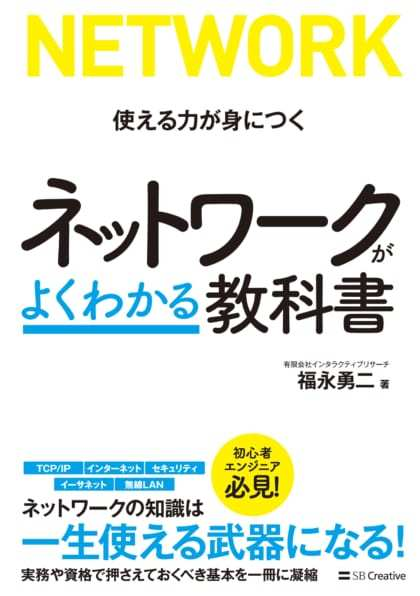
\includegraphics[width=4cm,bb=0 0 420 596]{./figures/networkbook.jpg}
      \label{fig:networkbook}
      \caption{テキスト}
    \end{figure}
  \end{minipage}

  \begin{itemize}
    \item 書影
    \begin{itemize}
      \item { \small \url{https://www.sbcr.jp/product/4797393804/} }
    \end{itemize}
  \end{itemize}

\end{frame}

\begin{frame}{今回の内容}

  \begin{itemize}
    \item TCP/IPの基本的な概念
      \begin{itemize}
        \item ネットワークプロトコル(TCP/IP 4階層モデル)
        \item インターネット層で使われるプロトコルの概要(IP、ICMP)
        \item トランスポート層で使われるプロトコルの概要(TCP、UDP)
        \item IPアドレス(p.44 ネットワークアドレスまで)
      \end{itemize}
    \item 徐々に掘り下げながら、といった構成なので今回は概要の説明が主
  \end{itemize}

\end{frame}


\begin{frame}{ネットワークプロトコル 1/3}

  \centering
  \begin{figure}
    \centering
    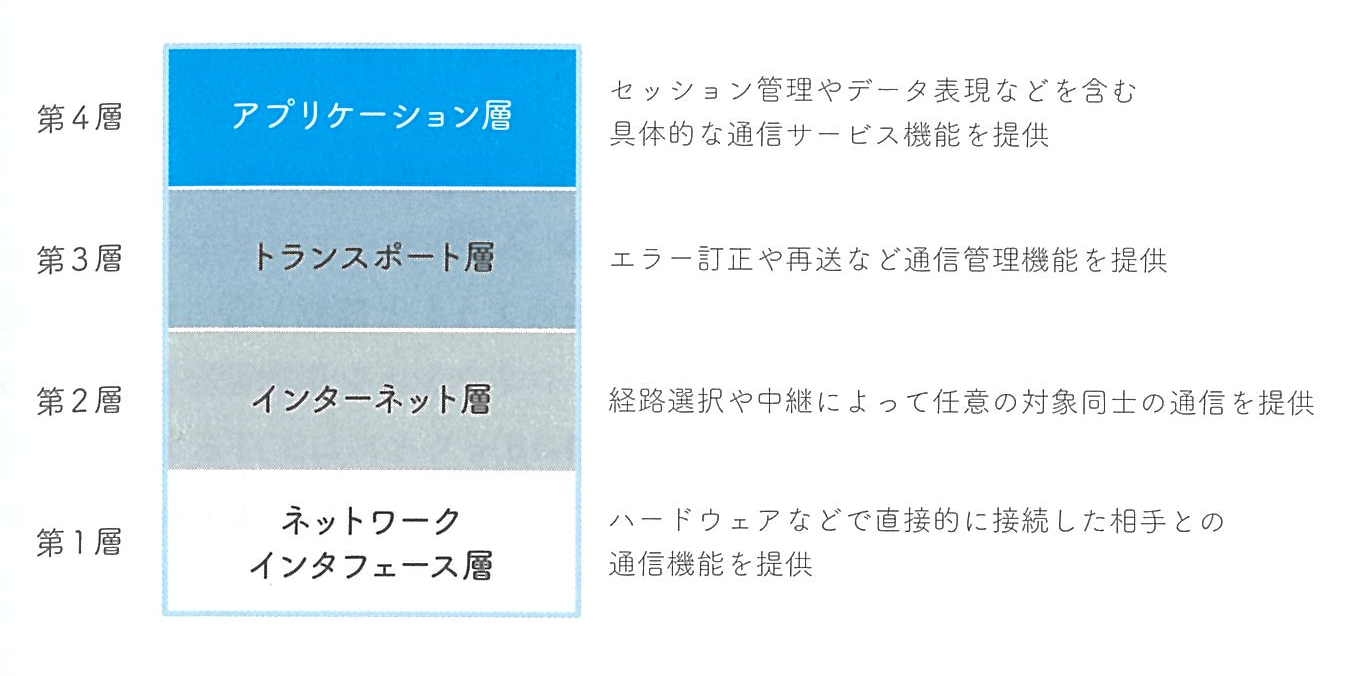
\includegraphics[width=12cm,bb=0 0 1352 676]{./figures/text_figure1_11.png}
    \label{fig:text_figure1_11}
    \caption{TCP/IP 4階層モデル(テキスト p.13より引用)}
  \end{figure}

\end{frame}


\begin{frame}{ネットワークプロトコル 2/3}

  \begin{itemize}
    \item TCP/IP 4階層モデル
      \begin{itemize}
        \item ネットワークインタフェース層(Chapter 3)
          \begin{itemize}
            \item 例:Ethernet
          \end{itemize}
        \item \textgt {インターネット層(Chapter 2)}
          \begin{itemize}
            \item 例:IP、ICMP
          \end{itemize}
        % https://ja.wikipedia.org/wiki/%E3%83%88%E3%83%A9%E3%83%B3%E3%82%B9%E3%83%9D%E3%83%BC%E3%83%88%E5%B1%A4
        \item \textgt {トランスポート層(Chapter 2)}
          \begin{itemize}
            \item 例:TCP、UDP、QUIC
          \end{itemize}
        % https://ja.wikipedia.org/wiki/%E3%82%A2%E3%83%97%E3%83%AA%E3%82%B1%E3%83%BC%E3%82%B7%E3%83%A7%E3%83%B3%E5%B1%A4
        \item アプリケーション層(Chapter 4以降)
          \begin{itemize}
            \item よく使われる例:HTTP、TLS、SSH、DNS、DHCP、NTP
            \item Eメール・メッセージ:IMAP、POP、SMTP、IRC、XMPP
            \item ファイル:FTP、SMB、NFS、WebDAV
          \end{itemize}

      \end{itemize}

    \item { \small 今回はインターネット層がメイン }

  \end{itemize}

\end{frame}


\begin{frame}{ネットワークプロトコル 3/3}

  \begin{itemize}
    \item インターネット層
      \begin{itemize}
        \item IP(Internet Protocol)
        \item ICMP(Internet Control Message Protocol)
      \end{itemize}

    \item トランスポート層
      \begin{itemize}
        \item TCP(Transmission Control Protocol)
        \item UDP(User Datagram Protocol)
        \item 余談:QUIC(Quick UDP Internet Connections)
          \begin{itemize}
            \item UDPをもとにしたプロトコル
            \item 従来アプリケーション層(TLS over TCP)で実装されていた暗号化をトランスポート層レベルでサポート(高速化に貢献)など
            % 一度TCPの接続を確立してからTLSの情報をやりとりしていた→接続の確立と同時に暗号化に必要な情報をやりとりできるようになる、往復、RTT
            \item 主要な通信であるTCPの高速な代替を目標にGoogleやIETFが実験・開発中
            % https://ja.wikipedia.org/wiki/QUIC
            % https://ja.wikipedia.org/wiki/Internet_Engineering_Task_Force
            % https://qiita.com/flano_yuki/items/251a350b4f8a31de47f5
          \end{itemize}
      \end{itemize}

    \item { \small 今回はIPの説明に少しだけ入る }

  \end{itemize}

\end{frame}


\begin{frame}{ネットワークインタフェース層}

  \begin{itemize}
    \item ネットワークインタフェース層の機能
      \begin{itemize}
        \item 同じネットワーク内でお互いに通信できるようにする
        \item 同じネットワーク
          \begin{itemize}
            \item LANケーブルやL2スイッチで直接コンピュータを接続した1つのネットワーク
            \item ルータは含まない
          \end{itemize}
        \item コンピュータは電気信号/電波や光信号でお互いにやり取りする
          \begin{itemize}
            \item NIC / Network Interface Card
            \item LANケーブル(RJ-45コネクタ)・Wi-Fi
          \end{itemize}
        \item 物理アドレス(MACアドレス)によって通信相手を特定する
        \item 詳しいことは第3章(次章)以降で

      \end{itemize}

  \end{itemize}

\end{frame}


\begin{frame}{インターネット層 1/2}

  \begin{itemize}
    \item インターネット層の機能
      \begin{itemize}
        \item 異なるネットワーク間でお互いに通信できるようにする
        \item 異なるネットワーク
          \begin{itemize}
            \item ルータやL3スイッチによって接続された2つ以上のネットワーク
            \item 「ネットワーク」の区切りはルータ
          \end{itemize}

        \item ネットワークを分割して互いに接続すること
          \begin{itemize}
            \item インターネットワーキング
          \end{itemize}
          % 第1章でメリットが語られている

      \end{itemize}

  \end{itemize}

\end{frame}


\begin{frame}{インターネット層 2/2}

  \begin{itemize}
    \item インターネット層の機能
      \begin{itemize}

        \item ルータはネットワークとネットワークをつなぐ
        \item 論理アドレス(IPアドレス)によって通信相手を特定する
          \begin{itemize}
            \item ルータはパケット(データ)に含まれるIPアドレスをもとに、どのネットワークに送るか判断する(パケットを中継する)
            \item パケットの中継をルーティングという
          \end{itemize}

      \end{itemize}

  \end{itemize}

\end{frame}


\begin{frame}{トランスポート層}

  \begin{itemize}
    \item トランスポート層の機能
      \begin{itemize}
        \item 通信の信頼性や速度を目的に応じて調節する
          \begin{itemize}
            \item 通信の前に相手に(インターネット層を通じて)到達できるか・通信できるか確認する(コネクション指向性)
            \item 破損したり失われたりしたパケットの再送
            \item 通信相手や経路の性能などを考慮したパケットの制御
          \end{itemize}

      \end{itemize}

  \end{itemize}

\end{frame}


\begin{frame}{プロトコルと層}

  \begin{itemize}
    \item プロトコル
      \begin{itemize}
        \item 各層の機能を実現するための通信のルール

      \end{itemize}

    \item 層
      \begin{itemize}
        \item 通信において必要とされる機能を分割する
        \item 通信の目的(求められる機能)に応じて層ごとにプロトコルを交換できる
        \item 異なる層でどのようなプロトコルが使われているかを(ある程度)無視できる

      \end{itemize}


  \end{itemize}

\end{frame}


\begin{frame}{インターネット層のプロトコル}

  \begin{itemize}
    \item インターネット層のプロトコル
      \begin{itemize}
        \item 異なるネットワーク間でお互いに通信できるようにする
        \item Internet Protocol(IP)
          \begin{itemize}
            \item 代表的なインターネット層のプロトコル
            \item IPアドレスの「IP」
            \item 主要なアプリケーションのデータのやり取りを行う
            \item バージョン:IPv4、IPv6
          \end{itemize}

        \item Internet Control Message Protocol(ICMP)
          \begin{itemize}
            \item ネットワーク機能を維持する裏方のプロトコル
            \item ネットワーク経路の検査や通信に使う制御情報のやり取りを行う(pingなど)
            \item IPパケットに含まれるデータとしてやりとりされるが、提供する機能の種類からインターネット層に分類される
          \end{itemize}

      \end{itemize}
  \end{itemize}

\end{frame}



\begin{frame}{トランスポート層のプロトコル 1/2}

  \begin{itemize}
    \item トランスポート層のプロトコル
      \begin{itemize}
        \item 通信の信頼性や速度を目的に応じて調節する
        \item TCP(Transmission Control Protocol)
          \begin{itemize}
            \item 代表的なトランスポート層のプロトコル
            \item 確実に相手に届ける(信頼性が高い)
            \item アプリケーションプロトコルの例:HTTP(Webページ)、POP/IMAP/SMTP(メール)など
          \end{itemize}

      \end{itemize}
  \end{itemize}

\end{frame}


\begin{frame}{トランスポート層のプロトコル 2/2}

  \begin{itemize}
    \item トランスポート層のプロトコル
      \begin{itemize}
        \item UDP(User Diagram Protocol)
          \begin{itemize}
            \item 相手に届くかどうか・届いたかどうかを確認しない(信頼性が低い)
            \item 速く相手に届ける(高速/低遅延の通信)
            \item アプリケーションプロトコルの例:DOMAIN(DNS)、NTP(時刻調整)、RTP(音声や動画のストリーミング)など
          \end{itemize}

      \end{itemize}
  \end{itemize}

\end{frame}


\begin{frame}{IPアドレス 1/2}

  \begin{itemize}
    \item IPアドレス
      \begin{itemize}
        \item インターネット層(ネットワーク間をつなぐ層)で使われる論理アドレス
        \item インターネットで使われるIPアドレスは重複しないように管理されている
          \begin{itemize}
            \item IANA(国際)をトップとする階層構造の組織
          \end{itemize}
      \end{itemize}

  \end{itemize}

\end{frame}


\begin{frame}{IPアドレス 2/2}

  \begin{figure}
    \centering
    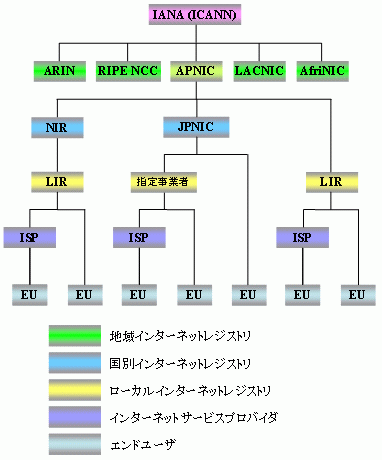
\includegraphics[width=5cm,bb=0 0 382 460]{./figures/ipreg.png}
    \label{fig:ipreg}
    \caption{IPアドレスの管理構造(JPNIC Webサイトより)}
  \end{figure}

  \centering
  { \small 引用:\url { https://www.nic.ad.jp/ja/ip/admin.html } }

\end{frame}


\begin{frame}{IPアドレスの種類 1/2}
  \begin{itemize}
    \item IPv4アドレス
      \begin{itemize}
        \item 32ビットの数値(だいたい\( 2^{32} \simeq 43 \)億個)
        \item 8ビット(1バイト)ずつに区切って4つの10進数で表示する
        \item UEC 学内ネットワーク: 130.153.0.0〜130.153.255.255(130.153.0.0/16)
        % 実験用ネットワークなどを除く
      \end{itemize}
    \item { \small 参考:\url { https://www.cc.uec.ac.jp/srv/infra/ip_manage.html } }

  \end{itemize}

\end{frame}


\begin{frame}{IPアドレスの種類 2/2}

  \begin{itemize}
    \item IPv6アドレス
      \begin{itemize}
        \item 128ビットの数値(だいたい\( (2^{32})^4 \simeq 3.4 \times 10^{38} \)個)
        \item 16ビット(2バイト)ずつに区切って8つの16進数で表示する
        \item UEC: 2001:02f8:0026:0000:0000:0000:0000:0000〜2001:02f8:0026:ffff:ffff:ffff:ffff:ffff(2001:02f8:0026::/48)
        \item 詳しくは第2章16節
      \end{itemize}
    \item { \small 参考:\url { https://www.cc.uec.ac.jp/srv/infra/ip_manage.html } }

  \end{itemize}

\end{frame}


\begin{frame}{IPアドレスの例}

  \begin{itemize}
    \item IPアドレスの例
      \begin{itemize}
        \item www.uec.ac.jp: 130.153.9.34
      \end{itemize}

  \end{itemize}

  \begin{figure}
    \centering
    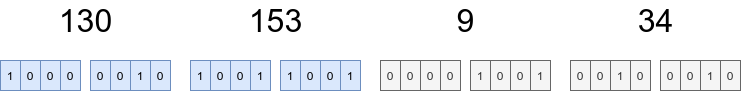
\includegraphics[width=12cm,bb=0 0 741 91]{./figures/ipaddr.png}
    \label{fig:ipaddr}
    \caption{電通大HPサーバのIPv4アドレス}
  \end{figure}

\end{frame}


\begin{frame}{IPアドレスの構成 1/2}

  \begin{itemize}
    \item IPアドレスは「ネットワーク部」と「ホスト部」から構成される
    \item ネットワーク部(左側)
      \begin{itemize}
        \item 目的地までの途中にあるルータがどのネットワークにパケットを送るかを決めるための部分
      \end{itemize}
    \item ホスト部(右側)
      \begin{itemize}
        \item 目的地のネットワークにあるルータがどのホスト(コンピュータ)にパケットを送るかを決めるための部分
      \end{itemize}
    \item ネットワーク部とホスト部にそれぞれ何ビット分をつかうかはIPアドレスによって異なる

  \end{itemize}

\end{frame}


\begin{frame}{IPアドレスの構成 2/2}

  \begin{itemize}
    \item 電通大HPサーバのIPアドレス
    \begin{itemize}
      \item 左側16ビット:ネットワーク部(青)
      \item 右側16ビット:ホスト部(灰)
    \end{itemize}
  \end{itemize}

  \begin{figure}
    \centering
    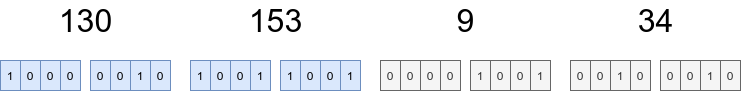
\includegraphics[width=12cm,bb=0 0 741 91]{./figures/ipaddr.png}
    \label{fig:ipaddr_re}
    \caption{電通大HPサーバのIPv4アドレス(再掲)}
  \end{figure}

\end{frame}


\begin{frame}{IPアドレスのクラス}

    \begin{itemize}
      \item IPアドレスはネットワーク部の長さによって分類される(クラス)
      \item ネットワーク部の長さはIPアドレスの先頭の数ビットで表される
      \item クラスA(8ビット)、クラスB(16ビット)、クラスC(24ビット)
      \begin{itemize}
        \item 特殊なIPアドレスとしてクラスD、Eもあるが省略
      \end{itemize}
    \end{itemize}

    \begin{figure}
      \centering
      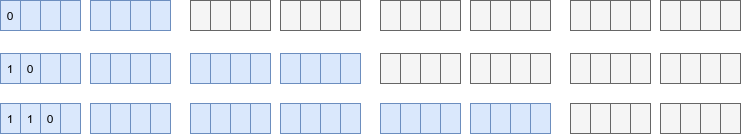
\includegraphics[width=12cm,bb=0 0 741 134]{./figures/ipblock_abc.png}
      \label{fig:ipblock_abc}
      \caption{クラスA、B、Cのネットワーク部の長さと先頭ビット}
    \end{figure}

\end{frame}


\begin{frame}{IPアドレスのクラスと収容できるネットワーク・ホスト数}

  \begin{itemize}
    \item クラスA:0.0.0.0〜127.255.255.255
      \begin{itemize}
        \item ネットワーク数:128ネットワーク(\( 2^{7} \))
        \item ホスト数:約1700万台(\( 2^{24} - 2 \))
      \end{itemize}
    \item クラスB:128.0.0.0〜191.255.255.255
      \begin{itemize}
        \item ネットワーク数:約17000ネットワーク(\( 2^{14} \))
        \item ホスト数:65534台(\( 2^{16} - 2 \))
      \end{itemize}
    \item クラスC:192.0.0.0〜223.255.255.255
      \begin{itemize}
        \item ネットワーク数:約200万ネットワーク(\( 2^{21} \))
        \item ホスト数:254台(\( 2^{8} - 2 \))
      \end{itemize}
    \item { \small ※ 最終桁が0または255の場合、特別な意味を持つためホストに使用できない }
  \end{itemize}

\end{frame}


\begin{frame}{ネットワークアドレス}

  \begin{itemize}
    \item ネットマスク
      \begin{itemize}
        \item IPアドレスとAND演算したときネットワーク部だけが得られるビット列(数値)
        \item AND演算の例:0b1011 \& 0b1101 = 0b1001
        \item クラスC ネットワークのネットマスク:255.255.255.0
        \item クラスB ネットワークのネットマスク:255.255.0.0
        \item 電通大HPサーバの属するネットワークのネットマスク:255.255.0.0
      \end{itemize}

    \item ネットワークアドレス
      \begin{itemize}
        \item ホスト部がすべて0でネットワーク部だけが含まれるIPアドレス
        \item ホストのIPアドレスとネットマスクをAND演算することでそのホストの属するネットワークアドレスが得られる
        \item ネットワーク自体を表し、これをホストに割り当てることはできない
        \item 電通大HPサーバのネットワークアドレス:130.153.0.0
      \end{itemize}

  \end{itemize}

\end{frame}


\begin{frame}{クラス別IPアドレスの問題点}

  \begin{itemize}
    \item 100台のコンピュータを含むネットワークを20個作りたい(ホスト2000台)
      \begin{itemize}
        \item クラスCのIPアドレスブロックが20個必要(ホスト5080台分)
      \end{itemize}

    \item 300台のコンピュータを含むネットワークを10個作りたい(ホスト3000台)
      \begin{itemize}
        \item クラスBのIPアドレスブロックが10個必要(ホスト655340台分)
      \end{itemize}

    \item 100000台のコンピュータを含むネットワークを3個作りたい(ホスト300000台)
      \begin{itemize}
        \item クラスAのIPアドレスブロックが3個必要(ホスト約5033万台分)
      \end{itemize}

    \item 使わないIPアドレスが発生する
    \item 多くのホストを接続することができるネットワークの数は限られている

  \end{itemize}

\end{frame}


\end{document}
